\section{Интуиционистское исчисление высказываний}
\begin{enumerate}
    \item (1 балл) Допишите указание истинности переменных в следующей шкале Крипке так,
    чтобы она опровергала формулу $(p \rightarrow q \lor r) \rightarrow (p \rightarrow q) \lor (p \rightarrow r)$:
    \begin{center}
        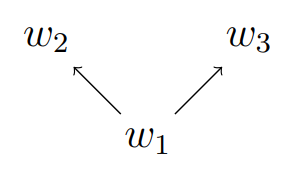
\includegraphics[width=0.15\textwidth]{hw05_1.png}
    \end{center}
    \begin{solution}
        Пусть в $w_2$ выводимо $p, q$, в $w_3$ выводимо $p, r$, тогда в $w_2$ и $w_2$ еще выводимо:
        \begin{equation}
            q \lor r
        \end{equation}
        В $w_1$ выводимо:
        \begin{equation}
            p \rightarrow q \lor r
        \end{equation}
        Но в $w_1$ не выводится
        \begin{align*}
            &p \rightarrow q \\
            &p \rightarrow r \\
            &(p \rightarrow q) \lor (p \rightarrow r)
        \end{align*}
        Поэтому опровержима формула $(p \rightarrow q \lor r) \rightarrow (p \rightarrow q) \lor (p \rightarrow r)$.
    \end{solution}
    \item (1 балл) Допишите указание истинности переменных в следующей шкале Крипке так,
    чтобы она опровергала формулу $(\overline{p} \rightarrow q \lor r) \rightarrow (\overline{p} \rightarrow q) \lor (\overline{p} \rightarrow r)$:
    \begin{center}
        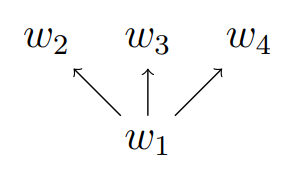
\includegraphics[width=0.15\textwidth]{hw05_2.png}
    \end{center}
    \begin{solution}
        Пусть в $w_2$ выводимо $p, q$, в $w_3$ выводимо $q$, в $w_4$ выводимо $r$ тогда в $w_2$, $w_3$ и $w_4$ еще выводимо:
        \begin{equation}
            q \lor r
        \end{equation}
        Пусть в $w_3$ и $w_4$ еще выводимо:
        \begin{equation}
            \overline{p}
        \end{equation}
        В $w_1$ выводимо:
        \begin{equation}
            \overline{p} \rightarrow q \lor r
        \end{equation}
        Но в $w_1$ не выводится
        \begin{align*}
            &\overline{p} \rightarrow q \\
            &\overline{p} \rightarrow r \\
            &(\overline{p} \rightarrow q) \lor (\overline{p} \rightarrow r)
        \end{align*}
        Поэтому опровержима формула $(\overline{p} \rightarrow q \lor r) \rightarrow (\overline{p} \rightarrow q) \lor (\overline{p} \rightarrow r)$.
    \end{solution}
    \item Постройте шкалы Крипке, опровергающие следующие формулы:
    \begin{itemize}
        \item[(a)] (1 балл) $(p \rightarrow q) \rightarrow \overline{p} \lor q$
        \item[(b)] (2 балл) $((p \rightarrow q) \rightarrow p) \rightarrow p$
    \end{itemize}
\end{enumerate}
\clearpage
